\documentclass[12pt, a4paper]{article}

% ===== 中文支持 =====
\usepackage[UTF8, zihao=-4]{ctex}

% ===== 页边距 =====
\usepackage[top=2.5cm, bottom=2.5cm, left=2.8cm, right=2.8cm]{geometry}

% ===== 字体 =====
\usepackage{fontspec}
\setmainfont{Times New Roman}

% ===== 行距 =====
\usepackage{setspace}
\setstretch{1.5}
\setlength{\parskip}{0pt}

% ===== 插图 =====
\usepackage{graphicx}
\usepackage{float}
\graphicspath{{./}}

% ===== 表格 =====
\usepackage{booktabs}
\usepackage{array}
\usepackage{makecell}
\usepackage{adjustbox}
\usepackage{multirow}

% ===== 数学 =====
\usepackage{amsmath, amssymb}

% ===== 图表编号 =====
\renewcommand{\thefigure}{\arabic{section}-\arabic{figure}}
\renewcommand{\thetable}{\arabic{section}-\arabic{table}}
\counterwithin{figure}{section}
\counterwithin{table}{section}

% ===== 图表标题格式 =====
\usepackage{caption}
\captionsetup{
  font=small,
  labelsep=space,
  justification=centering,
  aboveskip=6pt,
  belowskip=12pt
}
\captionsetup[table]{
  aboveskip=12pt,
  belowskip=6pt,
  position=above
}

% ===== 页眉页脚 =====
\usepackage{fancyhdr}
\setlength{\headheight}{15pt}
\pagestyle{fancy}
\fancyhf{}
\fancyhead[C]{\small 实验报告}
\fancyfoot[C]{\small\thepage}

% ===== 超链接 =====
\usepackage[colorlinks=true, linkcolor=black, citecolor=black, urlcolor=blue,
            bookmarks=true, bookmarksnumbered=true]{hyperref}

% ===== 章节标题 =====
\usepackage{titlesec}
\titleformat{\section}[block]
  {\centering\heiti\zihao{4}}{\thesection}{1em}{}
\titlespacing*{\section}{0pt}{24pt}{18pt}
\titleformat{\subsection}[hang]
  {\heiti\zihao{-4}}{\thesubsection}{1em}{}
\titlespacing*{\subsection}{0pt}{18pt}{6pt}
\titleformat{\subsubsection}[hang]
  {\heiti\zihao{-4}}{\thesubsubsection}{1em}{}
\titlespacing*{\subsubsection}{0pt}{12pt}{6pt}

\begin{document}

% ===== 封面 =====
\begin{titlepage}
  \centering
  \vspace*{3cm}
  {\heiti\zihao{2} 实验报告} \\[1cm]
  {\heiti\zihao{3} 望远镜与显微镜的设计与性能检测} \\[2cm]
  \begin{tabular}{ll}
    姓\quad 名： & 叶哲昊 \\[0.5cm]
    学\quad 号： & 24012561 \\[0.5cm]
    实验日期：   & 2026.4.24 \\
  \end{tabular}
  \vfill
\end{titlepage}

\tableofcontents
\newpage

\setcounter{page}{1}

% SECTION 1: 实验目的
\section{实验目的}

\begin{enumerate}
  \item 掌握望远镜的构造和工作原理。
  \item 了解测定望远镜的视角放大率和视场角的方法。
  \item 掌握显微镜的构造和工作原理。
  \item 了解显微镜放大倍数的测量原理和方法。
\end{enumerate}

% SECTION 2: 实验原理
\section{实验原理}

\subsection{望远镜}

\subsubsection{望远镜分类}

望远镜是帮助人眼对远处物体进行观察、瞄准与测量的助视光学仪器。常见望远镜分为\textbf{伽利略望远镜}（物镜为凸透镜，目镜为凹透镜，成正像，镜筒短但视场小）和\textbf{开普勒望远镜}（物镜和目镜均为凸透镜，成倒像，但视场大、可安装分划板），如图~\ref{fig:kepler}所示。

\begin{figure}[H]
  \centering
  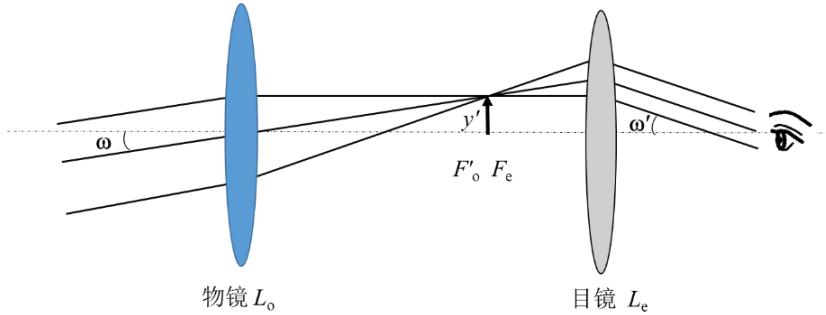
\includegraphics[width=0.85\textwidth]{images/791e1107baa8bf15b37384225cce4c9b0296d77f5cadfc7cbbb193b01b8ff554.jpg}
  \caption{开普勒望远镜光路示意图}
  \label{fig:kepler}
\end{figure}

远处射来的平行光经物镜会聚后，在物镜后焦面上成一倒立、缩小的实像，该像恰好落在目镜的前焦面上。人眼通过目镜观察时，最终成像于无穷远处，从而增大了视角，提高了分辨能力。

\subsubsection{视角放大率}

当观测无限远处的物体时，物镜的焦平面与目镜的焦平面重合。设光学仪器所成的像对人眼的张角为 $\omega'$，物体直接对人眼的张角为 $\omega$，则视角放大率定义为：

\begin{equation}
  \Gamma = \frac{\tan\omega'}{\tan\omega}
  \label{eq:gamma_def}
\end{equation}

由几何光路：
\begin{equation}
  \tan\omega = \frac{y'}{f_o'},\quad \tan\omega' = \frac{y'}{f_e'}
  \label{eq:tan_omega}
\end{equation}

因此望远镜的视角放大率为：
\begin{equation}
  \Gamma_T = \frac{f_o'}{f_e'}
  \label{eq:gamma_T}
\end{equation}

可见，望远镜的视角放大率等于物镜焦距与目镜焦距之比。

\subsubsection{物像共面时的视角放大率}

在实验室条件下，被观测物位于有限远处，可通过移动目镜将像推至与物 $y$ 共面来测量，如图~\ref{fig:coplanar}所示。

\begin{figure}[H]
  \centering
  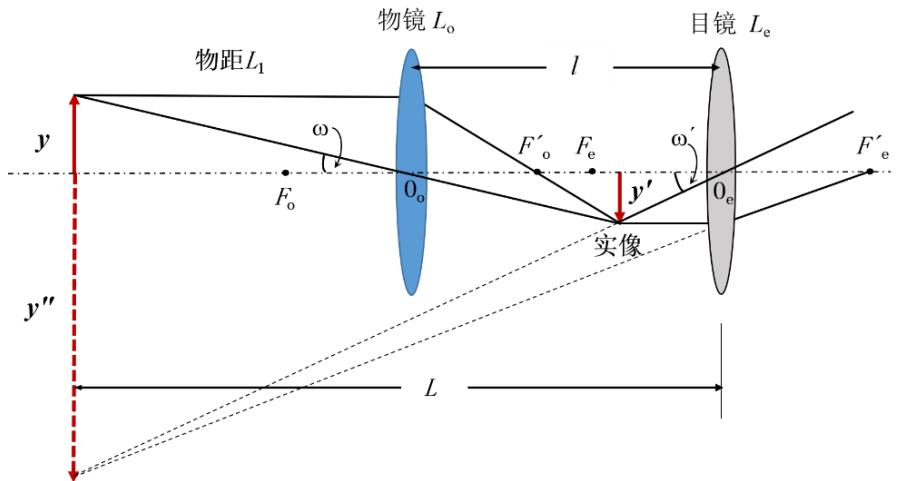
\includegraphics[width=0.85\textwidth]{images/7007526c1dbad0abfa10241127bfc4e433eb8f668930b38981bbea2f351f74f9.jpg}
  \caption{测望远镜物像共面时的视角放大率示意图}
  \label{fig:coplanar}
\end{figure}

此时 $\tan\omega' = y''/L$，$\tan\omega = y/L_1$，则物像共面时的视角放大率为：

\begin{equation}
  \Gamma_T = \frac{\tan\omega'}{\tan\omega} = \frac{y''}{L}\cdot\frac{L_1}{y}
           = \frac{L_1}{L}\cdot\frac{f_o'(L+f_e')}{f_e'(L_1-f_o')}
  \label{eq:gamma_coplanar}
\end{equation}

当物距 $L_1$ 大于20倍物镜焦距 $f_o'$ 时，该值与无穷远时的视角放大率差别很小。

\subsection{显微镜}

\subsubsection{显微镜简介}

显微镜用于观察近处的微小物体，其光学系统由焦距较短的物镜 $L_o$ 和目镜 $L_e$ 组成，均为会聚透镜，如图~\ref{fig:microscope_basic}所示。位于物镜物方焦点附近（一倍至二倍焦距之间）的微小物体，经物镜放大后先成一放大实像，此实像再经目镜进一步放大，最终成像于无穷远处（或明视距离处），实现两次放大。

\begin{figure}[H]
  \centering
  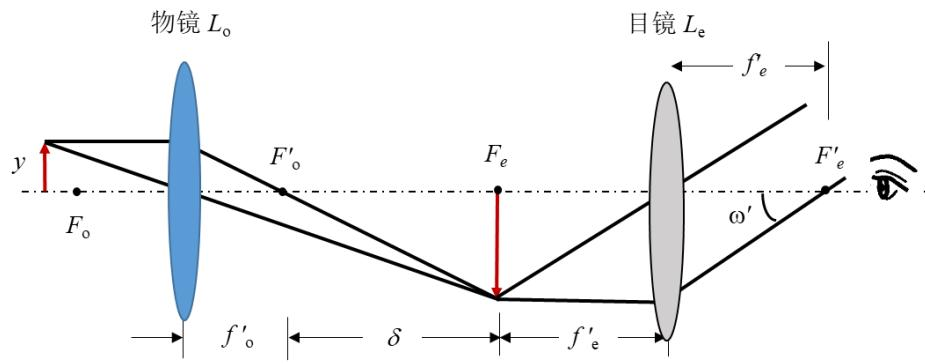
\includegraphics[width=0.80\textwidth]{images/34076f98cfdc514855cbbcd13054554f93f29e4bc8fafb07befdbd87847da377.jpg}
  \caption{显微镜基本光学系统}
  \label{fig:microscope_basic}
\end{figure}

\subsubsection{显微镜的视角放大率}

显微镜视角放大率定义为像对人眼张角的正切与物在明视距离 $D=250\,\text{mm}$ 处直接对人眼张角的正切之比：

\begin{equation}
  \Gamma_M = \frac{y'/f_e'}{y/D} = \frac{Dy'}{f_e' y} = \frac{D\delta}{f_e' f_o'} = \beta_o\,\Gamma_e
  \label{eq:gamma_M}
\end{equation}

其中 $\beta_o = y'/y = \delta/f_o'$ 为物镜的线放大率，$\Gamma_e = D/f_e'$ 为目镜的视角放大率，$\delta$ 为光学间隔。由此可见，物镜和目镜焦距越短、光学间隔越大，显微镜放大倍数越大。

\subsubsection{成像于有限远时的视角放大率}

当显微镜成虚像于距目镜为 $l''$ 的位置上，人眼在目镜后焦点处观察时，视角放大率仍为：

\begin{equation}
  \Gamma_M = \frac{y''/(l''+f_e')}{y/D} = \beta_o\,\Gamma_e
  \label{eq:gamma_M_finite}
\end{equation}

中间像不在目镜物方焦平面上时，$\beta_o = y'/y \neq \delta/f_o'$。此时可借助与主光轴成 $45°$ 放置的半透半反镜（分束镜），将毫米标尺成虚像至显微镜的像平面，直接比较测量像长 $y''$，从而得到视角放大率：

\begin{equation}
  \Gamma_M = y''/y
  \label{eq:gamma_M_measure}
\end{equation}

有限远成像时的显微镜光路如图~\ref{fig:microscope_finite}所示。

\begin{figure}[H]
  \centering
  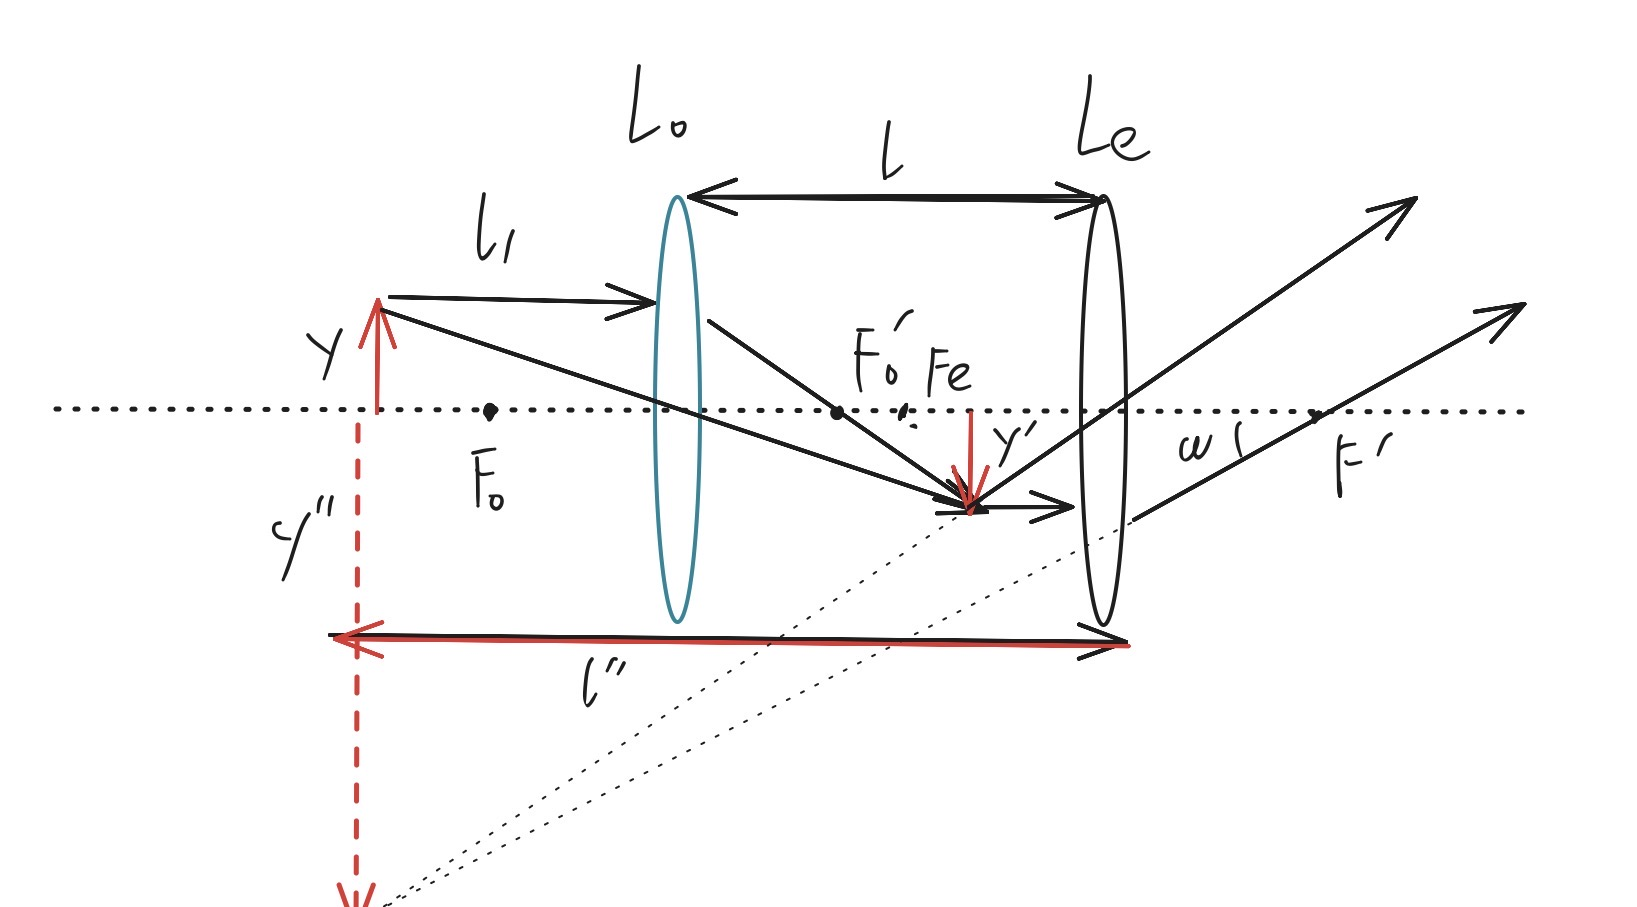
\includegraphics[width=0.85\textwidth]{images/microscope_finite_imaging_correct.jpg}
  \caption{显微镜成像于有限远时的光路图（物体位于物镜一倍至二倍焦距之间）}
  \label{fig:microscope_finite}
\end{figure}

% SECTION 3: 实验仪器
\section{实验仪器}

\subsection{望远镜实验}

\begin{itemize}
  \item 目镜：直径 $\phi=20\,\text{mm}$，焦距 $f_e'=30\,\text{mm}$
  \item 物镜：直径 $\phi=40\,\text{mm}$，焦距 $f_o'=150\,\text{mm}$
  \item 毫米标尺
\end{itemize}

\subsection{显微镜实验}

\begin{itemize}
  \item 分束镜（与主光轴成 $45°$ 放置）
  \item 目镜：直径 $\phi=20\,\text{mm}$，焦距 $f_e'=30\,\text{mm}$
  \item 物镜：直径 $\phi=50\,\text{mm}$，焦距 $f_o'=75\,\text{mm}$
  \item 分辨率板（United States Air Force 1951 分辨率测试卡）
  \item LED 光源（含匀光器）×2
  \item 毫米标尺
\end{itemize}

% SECTION 4: 实验步骤
\section{实验步骤}

\subsection{望远镜实验}

\begin{enumerate}
  \item 在导轨上依次放置目镜（$f_e'=30\,\text{mm}$）、物镜（$f_o'=150\,\text{mm}$）和毫米标尺。目标标尺与物镜间的距离要求大于2倍物镜焦距（即 $L_1>300\,\text{mm}$）。

  \item 用一只眼通过目镜观察标尺的像，移动目镜使之聚焦清晰；同时用另一只眼直接观察标尺。适应性练习后，调整至两眼视场中望远镜的标尺放大像与直接观察到的标尺基本重合，且无视差。

  \item 在视场中同时看到标尺原像（左）和放大像（右），如图~\ref{fig:scale_view}所示，读取像格数 $n$ 所对应的标尺格数 $m$，计算放大率实验值 $\Gamma_i = m/n$，重复测量3次。

  \begin{figure}[H]
    \centering
    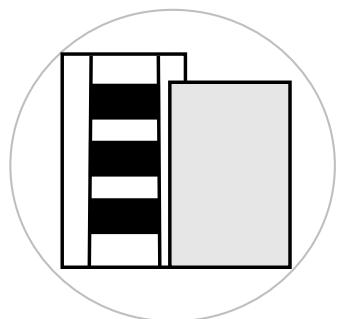
\includegraphics[width=0.60\textwidth]{images/3bf3fc7fc9b01dbcc2c7c1c6c7118df77552c5dbeb764adf6b165804e76fc150.jpg}
    \caption{目镜视场中标尺（左）与放大像（右）示意图}
    \label{fig:scale_view}
  \end{figure}

  \item 测量物距 $L_1$（标尺到物镜）和像距 $L$（目镜到标尺像面），代入公式（\ref{eq:gamma_coplanar}）计算理论放大率，并与实验值比较。
\end{enumerate}

\subsection{显微镜实验}

\begin{enumerate}
  \item 在导轨上依次放置分束镜（$45°$ 反射角）、目镜（$f_e'=30\,\text{mm}$）、物镜（$f_o'=75\,\text{mm}$）、分辨率板、LED光源（含匀光器）。导轨外由远及近依次放置LED光源（含匀光器）和毫米标尺，标尺位于距分束镜明视距离（$250\,\text{mm}$）处。如图~\ref{fig:microscope_setup}所示。

  \begin{figure}[H]
    \centering
    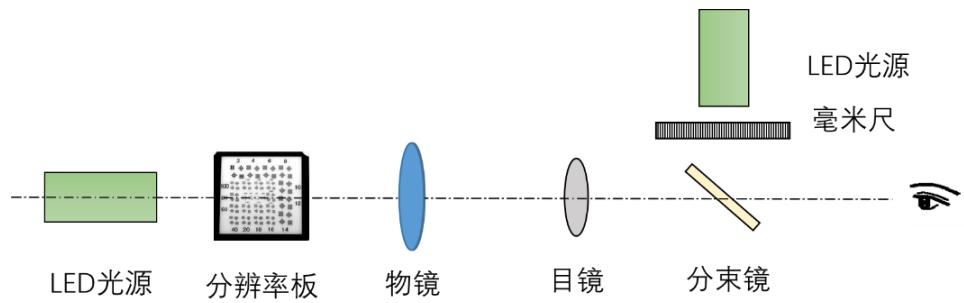
\includegraphics[width=0.85\textwidth]{images/1a784668db3e0ae9d933afd9a43ba4f7858570a9674a80d26e51b67872439aae.jpg}
    \caption{测显微镜视角放大率实际光路图（人眼紧贴分束镜观察）}
    \label{fig:microscope_setup}
  \end{figure}

  \item 调整分辨率板与物镜之间的距离，使其介于物镜的一倍焦距和二倍焦距之间（$75\,\text{mm} < l_1 < 150\,\text{mm}$）。

  \item 调整观察位置，在视野中同时观察到分辨率板的条纹和毫米标尺的刻度像，如图~\ref{fig:fov}所示。

  \begin{figure}[H]
    \centering
    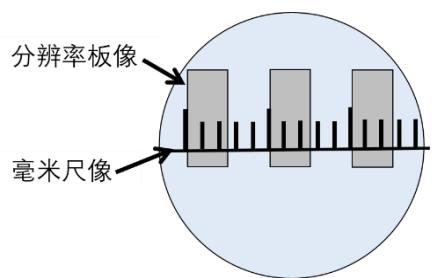
\includegraphics[width=0.55\textwidth]{images/42c3652e0d0bfd259b31ac58c858163f2ed692de6ec51590ba950b422889a950.jpg}
    \caption{视野中分辨率板像（条纹）和毫米标尺像}
    \label{fig:fov}
  \end{figure}

  \item 在视场中寻找4号条纹的清晰像，通过标尺刻度测定条纹像宽度 $d'$，重复测量3次。根据实际宽度 $d=0.25\,\text{mm}$ 计算放大倍数实验值 $\Gamma=d'/d$。

  \item 测量物距 $l_1$（分辨率板到物镜），由薄透镜成像公式计算像距 $q_o$，进而求物镜放大率 $\beta_o$ 和目镜放大率 $\Gamma_e$，计算理论总放大率。
\end{enumerate}

% SECTION 5: 实验数据与处理
\section{实验数据与处理}

\subsection{望远镜实验}

\subsubsection{视角放大率测量}

仪器参数：物镜焦距 $f_o'=150\,\text{mm}$，目镜焦距 $f_e'=30\,\text{mm}$；像格数固定 $n=1$ 格。

\begin{table}[H]
  \caption{表~5-1\quad 望远镜视角放大率测量记录（物像共面法）}
  \label{tab:telescope}
  \centering
  \begin{adjustbox}{max width=\textwidth}
    \begin{tabular}{ccccc}
      \toprule
      测量序号 & 物格数 $m$ & 像格数 $n$ & 放大率实验值 $\Gamma_i = m/n$ & 备注 \\
      \midrule
      1 & 7 & 1 & 7 & \\
      2 & 6 & 1 & 6 & \\
      3 & 6 & 1 & 6 & \\
      \midrule
      平均值 & \multicolumn{2}{c}{——} & $\bar{\Gamma}_e = 6.333$ & \\
      \bottomrule
    \end{tabular}
  \end{adjustbox}
\end{table}

\subsubsection{理论放大率计算}

测量得到：物距 $L_1 = 900\,\text{mm}$（标尺到物镜），像距 $L = 1106\,\text{mm}$（目镜到标尺像面）。

代入公式（\ref{eq:gamma_coplanar}）计算理论放大率：

\begin{align}
  \Gamma &= \frac{L_1}{L}\cdot\frac{f_o'(L+f_e')}{f_e'(L_1-f_o')} \notag\\[6pt]
         &= \frac{900}{1106}\times\frac{150\times(1106+30)}{30\times(900-150)} \notag\\[6pt]
         &= \frac{900}{1106}\times\frac{150\times 1136}{30\times 750} \notag\\[6pt]
         &= 0.8137\times 7.5733 = 6.163
  \label{eq:telescope_theory}
\end{align}

相对偏差：
\begin{equation}
  E = \frac{\bar{\Gamma}_e - \Gamma}{\Gamma}\times 100\%
    = \frac{6.333 - 6.163}{6.163}\times 100\%
    = 2.768\%
  \label{eq:E_telescope}
\end{equation}

\subsection{显微镜实验}

\subsubsection{视角放大率测量}

仪器参数：物镜焦距 $f_o'=75\,\text{mm}$，目镜焦距 $f_e'=30\,\text{mm}$，明视距离 $D=250\,\text{mm}$；
被测对象：4号条纹，实际黑条宽度 $d=0.25\,\text{mm}$。

\begin{table}[H]
  \caption{表~5-2\quad 显微镜视角放大率测量记录（分束镜比较法）}
  \label{tab:microscope}
  \centering
  \begin{adjustbox}{max width=\textwidth}
    \begin{tabular}{cccc}
      \toprule
      测量序号（4号） & 条纹实际宽度 $d$/mm & 条纹像宽度 $d'$/mm & 放大率实验值 $\Gamma_{\text{实验}} = d'/d$ \\
      \midrule
      1 & 0.25 & 2.9  & 11.6 \\
      2 & 0.25 & 2.8  & 11.2 \\
      3 & 0.25 & 2.8  & 11.2 \\
      \midrule
      平均值 & 0.25 & $\bar{d}' = 2.833$ & $\bar{\Gamma}_{\text{实验}} = 11.333$ \\
      \bottomrule
    \end{tabular}
  \end{adjustbox}
\end{table}

\subsubsection{理论放大率计算}

测量得物距 $l_1 = 135\,\text{mm}$（分辨率板到物镜，取绝对值；在 $75\,\text{mm}$ 与 $150\,\text{mm}$ 之间，满足要求）。

\textbf{物镜像距 $q_o$（由薄透镜成像公式，使用实符号 $l_1$ 取负值 $l_1 = -135\,\text{mm}$）：}

\begin{equation}
  \frac{1}{q_o} = \frac{1}{f_o'} + \frac{1}{l_1}
               = \frac{1}{75} + \frac{1}{-135}
               = \frac{135 - 75}{75\times 135}
               = \frac{60}{10125}
  \quad\Rightarrow\quad q_o = \frac{10125}{60} = 168.75\,\text{mm}
  \label{eq:qo}
\end{equation}

\textbf{物镜放大率 $\beta_o$：}
\begin{equation}
  \beta_o = \frac{q_o}{|l_1|} = \frac{168.75}{135} = 1.25
  \label{eq:beta_o}
\end{equation}

\textbf{目镜放大率 $\Gamma_e$：}
\begin{equation}
  \Gamma_e = \frac{D}{f_e'} = \frac{250}{30} = 8.333
  \label{eq:gamma_e}
\end{equation}

\textbf{理论总放大率：}
\begin{equation}
  \Gamma = \beta_o\times\Gamma_e = 1.25\times 8.333 = 10.417
  \label{eq:gamma_theory_micro}
\end{equation}

\textbf{相对偏差：}
\begin{equation}
  E = \frac{\bar{\Gamma}_{\text{实验}} - \Gamma}{\Gamma}\times 100\%
    = \frac{11.333 - 10.417}{10.417}\times 100\%
    = 8.8\%
  \label{eq:E_microscope}
\end{equation}

% SECTION 6: 实验结果与分析
\section{实验结果与分析}

\subsection{望远镜实验结果}

望远镜实验结果汇总如下：

\begin{table}[H]
  \caption{表~6-1\quad 望远镜视角放大率实验结果汇总}
  \label{tab:telescope_result}
  \centering
  \begin{adjustbox}{max width=\textwidth}
    \begin{tabular}{lll}
      \toprule
      量\quad 名 & 数值 & 备注 \\
      \midrule
      放大率实验平均值 $\bar{\Gamma}_e$ & 6.333 & 三次测量平均 \\
      理论放大率 $\Gamma$（公式计算）& 6.163 & 由公式（\ref{eq:gamma_coplanar}）计算 \\
      理想放大率 $f_o'/f_e'$ & $150/30 = 5.000$ & 无穷远物体 \\
      相对偏差 $E$ & $2.768\%$ & \\
      \bottomrule
    \end{tabular}
  \end{adjustbox}
\end{table}

实验值 $\bar{\Gamma}_e = 6.333$ 与物像共面时理论值 $\Gamma = 6.163$ 的相对偏差为 $2.768\%$，两者符合良好。实验值略大于理论值，与随机读数误差有关。注意到物像共面时的理论放大率（6.163）大于无穷远物体情况下的理想放大率（5.000），这是因为物体置于有限距离时，物距 $L_1=900\,\text{mm}$ 仅为物镜焦距的6倍，有限距离效应使放大率偏高。

\subsection{显微镜实验结果}

显微镜实验结果汇总如下：

\begin{table}[H]
  \caption{表~6-2\quad 显微镜视角放大率实验结果汇总}
  \label{tab:microscope_result}
  \centering
  \begin{adjustbox}{max width=\textwidth}
    \begin{tabular}{lll}
      \toprule
      量\quad 名 & 数值 & 备注 \\
      \midrule
      条纹像宽度平均值 $\bar{d}'$ & $2.833\,\text{mm}$ & 三次测量平均 \\
      放大率实验平均值 $\bar{\Gamma}_{\text{实验}}$ & 11.333 & $\bar{d}'/d$ \\
      物镜放大率 $\beta_o$ & 1.25 & \\
      目镜放大率 $\Gamma_e$ & 8.333 & \\
      理论总放大率 $\Gamma$ & 10.417 & $\beta_o\times\Gamma_e$ \\
      相对偏差 $E$ & $8.8\%$ & \\
      \bottomrule
    \end{tabular}
  \end{adjustbox}
\end{table}

显微镜实验值 $\bar{\Gamma}_{\text{实验}} = 11.333$，理论值 $\Gamma = 10.417$，相对偏差为 $8.8\%$。实验值高于理论值，原因分析见第~\ref{sec:error}节。

% SECTION 7: 误差分析
\section{误差分析}
\label{sec:error}

\subsection{望远镜实验误差分析}

\begin{enumerate}
  \item \textbf{读数误差}：物像共面法需同时用双眼观察，需要一定的适应性训练，两眼视场的重合调整存在主观判断误差，导致 $m$ 值读数不稳定（本实验三次读数分别为 7、6、6）。

  \item \textbf{测距误差}：物距 $L_1$ 和像距 $L$ 均通过导轨刻度盘测量，导轨精度和各元件参考面定位引入系统误差。

  \item \textbf{视差误差}：双眼观察时若物像未能严格共面，会引入视差，从而系统性地偏高实验值。

  \item \textbf{像差}：实际透镜存在球差、色差等，导致成像质量下降，影响读数精度。
\end{enumerate}

\subsection{显微镜实验误差分析}

\begin{enumerate}
  \item \textbf{条纹像宽度读数误差}：分束镜将毫米标尺成虚像与显微镜像叠加，由于两路光强不均衡，条纹边缘与标尺刻线判读存在一定主观误差，这是显微镜相对偏差（$8.8\%$）较望远镜（$2.768\%$）偏大的主要原因。

  \item \textbf{物距测量误差}：物距 $l_1$ 的测量精度直接影响物镜像距 $q_o$ 的计算，从而影响理论放大率。实验中 $l_1=135\,\text{mm}$ 接近二倍焦距（$2f_o'=150\,\text{mm}$），在此范围内 $\beta_o$ 对 $l_1$ 的变化较敏感。

  \item \textbf{分束镜引入的光程差}：分束镜的厚度会引入额外光程，使明视距离的实际值与标准明视距离（$250\,\text{mm}$）略有偏差。

  \item \textbf{像差与衍射}：物镜和目镜的球差、色差以及衍射极限，会造成像的模糊，影响条纹像宽度的准确读取。
\end{enumerate}

% SECTION 8: 实验结论
\section{实验结论}

\begin{enumerate}
  \item \textbf{望远镜}：成功搭建了开普勒望远镜系统（$f_o'=150\,\text{mm}$，$f_e'=30\,\text{mm}$）。采用物像共面法测得视角放大率实验值 $\bar{\Gamma}_e = 6.333$，由公式计算的理论值 $\Gamma = 6.163$，相对偏差 $E = 2.768\%$，两者吻合较好，验证了望远镜视角放大率等于物镜焦距与目镜焦距之比这一结论。

  \item \textbf{显微镜}：成功搭建了含分束镜的显微镜测量系统（$f_o'=75\,\text{mm}$，$f_e'=30\,\text{mm}$）。采用分束镜比较法测得视角放大率实验值 $\bar{\Gamma}_{\text{实验}} = 11.333$，理论值 $\Gamma = \beta_o\times\Gamma_e = 1.25\times 8.333 = 10.417$，相对偏差 $E = 8.8\%$。实验验证了显微镜总放大率等于物镜线放大率与目镜视角放大率之积这一结论。

  \item 两个实验的相对偏差均在合理范围内，主要误差来源是目视读数的主观误差及光学元件的像差。总体而言，实验结果与理论预测符合良好，达到了实验目的。
\end{enumerate}

% SECTION 9: 思考题
\section{思考题}

\subsection*{思考题1}

\textit{开普勒望远镜和显微镜均由两个凸透镜组成，提高望远镜的放大率可通过增大物镜焦距或减小目镜焦距实现；但提高显微镜的放大率却是选用焦距较短的物镜和目镜，请说明原因。}

\textbf{答：}

两者放大率的决定因素不同：

\begin{itemize}
  \item \textbf{望远镜}：视角放大率 $\Gamma_T = f_o'/f_e'$。增大物镜焦距 $f_o'$ 或减小目镜焦距 $f_e'$，均可提高放大率。望远镜的物距趋于无穷远，物镜焦距越长，所成的中间实像越大（角放大），因此选用长焦距物镜有利。

  \item \textbf{显微镜}：视角放大率 $\Gamma_M = \beta_o\cdot\Gamma_e = \dfrac{\delta}{f_o'}\cdot\dfrac{D}{f_e'}$，与物镜和目镜的焦距均成反比。这是因为显微镜的物体置于物镜的一倍至二倍焦距之间，物镜作为放大镜起二次线放大作用，焦距越短，同样的光学间隔 $\delta$ 下物镜线放大率 $\beta_o = \delta/f_o'$ 越大；目镜焦距越短，目镜视角放大率 $\Gamma_e = D/f_e'$ 越大。因此，提高显微镜放大率需要同时选用短焦物镜和短焦目镜。
\end{itemize}

本质区别在于：望远镜的物位于无穷远，中间像大小由物方视角决定，增大物镜焦距能增大像的线尺寸；而显微镜的物是有限距离的微小物体，物镜本身作为放大系统，焦距越短放大倍数越高，两者的光学功能结构根本不同。

\subsection*{思考题2}

\textit{利用工程光学知识，试推导公式（2-3-4）和（2-3-5）。}

\textbf{答：}

\textbf{推导公式（2-3-4）—— 望远镜物像共面时的视角放大率：}

设标尺物高为 $y$，置于距物镜 $L_1$ 处；目镜中所成的最终虚像（通过整个望远镜系统）与标尺共面，像高为 $y''$，两者均在距人眼 $L$ 处。

由视角放大率定义：
\begin{equation*}
  \Gamma_T = \frac{\tan\omega'}{\tan\omega} = \frac{y''/L}{y/L_1} = \frac{y''}{y}\cdot\frac{L_1}{L}
\end{equation*}

对物镜，由高斯公式，物距 $-L_1$（实物取负），像距 $q_o$：
\begin{equation*}
  \frac{1}{q_o} - \frac{1}{-L_1} = \frac{1}{f_o'} \quad\Rightarrow\quad q_o = \frac{f_o' L_1}{L_1 - f_o'}
\end{equation*}

物镜成像高度：$y' = -\dfrac{q_o}{L_1}\,y = -\dfrac{f_o'}{L_1 - f_o'}\,y$

此中间像作为目镜物，物距为 $l_e = q_o - (L - f_e') \approx q_o$ 处（目镜成虚像到物面共面处）；由目镜成像：

目镜物距（取为 $l_e = -(L+f_e')$ 的适当形式，由几何关系）给出像高：
\begin{equation*}
  y'' = -\frac{f_e'}{l_e + f_e'}\,y' \cdot\frac{l_e + f_e'}{f_e'} = \frac{L+f_e'}{f_e'}\,\left|\frac{f_o'}{L_1-f_o'}\right|\,y
\end{equation*}

代入放大率：
\begin{equation*}
  \Gamma_T = \frac{y''}{y}\cdot\frac{L_1}{L}
           = \frac{f_o'(L+f_e')}{f_e'(L_1-f_o')}\cdot\frac{L_1}{L}
\end{equation*}

这即为公式（2-3-4）。

\textbf{推导公式（2-3-5）—— 显微镜成虚像于有限远时的视角放大率：}

设物高 $y$，物镜成中间实像高度 $y'$，此中间像再经目镜成虚像于距目镜 $l''$ 处（人眼于目镜后焦点 $f_e'$ 处观察），最终虚像高度 $y''$。

视角放大率：
\begin{equation*}
  \Gamma_M = \frac{\tan\omega'}{\tan\omega} = \frac{y''/(l''+f_e')}{y/D}
\end{equation*}

由目镜成像，对以 $y'$ 为物的目镜：
\begin{equation*}
  \frac{1}{-l''} - \frac{1}{l_e'} = \frac{1}{f_e'} \quad\Rightarrow\quad l_e' = \frac{f_e'\,l''}{l'' - f_e'}
\end{equation*}

横向放大率：$y''/y' = l''/(l''-f_e') \cdot(-) $，于是 $y''/(l''+f_e')$ 可化简。由薄透镜成像比例关系，最终化简结果为：

\begin{equation*}
  \Gamma_M = \frac{y''}{l''+f_e'}\cdot D = \frac{y'}{f_e'}\cdot\frac{D\,y'}{y\,y'} = \frac{D\,y'}{f_e'\,y} = \beta_o\,\Gamma_e
\end{equation*}

其中 $\beta_o = y'/y$ 为物镜线放大率，$\Gamma_e = D/f_e'$ 为目镜视角放大率。

可见，即使中间像不在目镜前焦面（即 $\beta_o \neq \delta/f_o'$），显微镜的视角放大率仍等于 $\beta_o\cdot\Gamma_e$，这一结论与无穷远成像情况一致，具有普遍性。

\end{document}
